I dette kapitel vil den initierende problemstilling blive analyset. Dette bliver gjort i form af en interessesentanalyse, hvor de væsentlige interessenter bliver fundet. På baggrund af interessentanalysen blev der sendt et spørgeskema ud, og et interview blev foretaget med VisitAalborg. Til slut er et par eksisterende løsninger blevet inddraget i dette kapitel. 

\section{Interessentanalyse}
Gruppen vil i dette afsnit, kigge på diverse personer/grupper, der kan fungere som interessenter i projektet, altså en person der vil have nytte af projektet. Herefter vil gruppen prioritere disse interessenter, alt efter hvor relevante de er i forhold til projektet.

\textbf{Turister}\newline
Turister er en væsentlig interessent i projektet, da en turist ofte vil se hvad byen har at byde på, eller nogle unikke attraktioner, i forhold til følgende citat: \newline 
\textit{“If you want visitors to come back again — and say nice things about your town to others who might come, too — you need to have some good answers at the ready. That means offering things to see and do that are either unique or extraordinary…”} \citep{UniversityOfMinnesota}.\newline 
Hvis turisterne planlægger hvad det er, de vil se, kan turisterne spare tid \citep{YouthCentral}. Turisterne kan vælge at gå en længere rute, og derved have mulighed for at finde andre ting, som de vælger at bruge deres tid på. Et ruteplanlægningsværktøj vil derfor være interessant for turister, da de derved kan komme til at besøge alle de attraktioner/seværdigheder, som de ønsker.
En-dagsturister er en mindre interessent i projektet, da en en-dagsturist maksimum overnatter en nat, og generelt har et formål med rejsen, som fx at besøge en attraktion, venner/familie eller er på et kursusophold \citep{Faxe}.

\textbf{Staten}\newline
Staten er en interessent i projektet. Hvis der er nogle unikke eller ekstraordinære attraktioner i en by, vil turister huske disse, som gode oplevelser, og nogle vil derfor komme igen. Det er noget som staten er interesseret i, da der kommer flere penge ind i landet \citep{VisitAalborg}.
Her vil et ruteplanlægningsværktøj kunne hjælpe turister med at se nogle af de attraktioner der er i landet, hvis der fx er en top 5 over de attraktionerne der er i landet, eller i den by ferien foregår.

\textbf{Retail-handel}\newline
Diverse forretninger er også interessenter i projektet, da kendte brands som fx IKEA, Bilka og lignende lever af deres kunder \citep{PengeloseButikker}. Ved at implementere disse adresser, i et ruteplanlægningsværktøj, kan det tiltrække turister, og derved øge omsætningen. 

\textbf{VisitAalborg}\newline
VisitAalborgs arbejde består af at støtte lokale aktører eller andre aktører, hvis disse aktører byder på nogle turistfremmende aktiviteter/projekter, der har til formål, at hjælpe Aalborg. Det kan fx være at henvise til aktørernes hjemmesider, gennem deres egen hjemmeside, der bliver set af ca. 600.000 årligt. \citep{VA}
Til et ruteplanlægningsværktøj er VisitAalborg en vigtig interessent, da de har informationer om turisterne i Aalborg. Ved at inddrage turistkontoret i projektet, vil gruppen gøre brug af deres ressourcer. 

\subsection{Prioriteringen}
For at prioritere interessenterne i projekter, og finde de vigtige interessenter, har gruppen valgt gøre brug af indflydelse/medvirken-matrixen, som kan ses på figur 2.1 herunder.

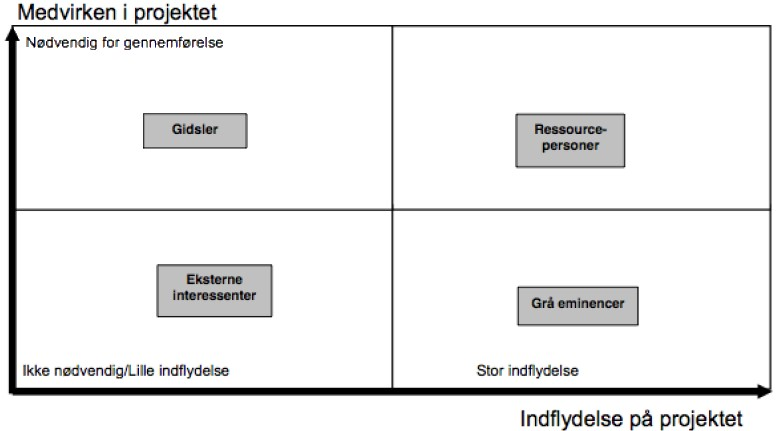
\includegraphics[scale=0.8]{Prior}
\textit{Figur 2.1: Indflydelse/medvirken-matrixen}\newline
 

Gidslerne i projektet, er staten og turisterne. Disse interessenter er blevet kategoriseret som gidsler, da deres indflydelse ikke er vigtig for at gennemføre projektet, men alligevel har de nogle informationer/ressourcer som skal bruges i projektet.

VisitAalborg i dette projekt er ressourceperson, da de har informationer om turister. Derudover kan turistkontoret komme med råd og vejledning for, at en eventuel løsning vil være mest op-timal for turisterne.   

De eksterne i projektet er retail-forretningerne. Deres indflydelse og medvirken er ikke nød-vendig, for at kunne gennemføre projektet. 

Gruppen har i dette projekt, ikke nogle interessenter der passer ind under kategorien grå emmi-nence. 

\subsection{Opsummering}
Ud fra interessentanalysen, er gruppen nået frem til, at VisitAalborg er ressourceperson, hvilket gruppen ser som en central interessent i projektet. Det er en nødvendig kilde, for at få nogle brugbare ressourcer. En anden central interessent, er turisterne, da det er dem, der skal gøre brug af ruteplanlægningsværktøjet. 
De andre interessenter, som gruppen har fundet frem til, er blevet vurderet som mindre vigtige, og derfor vil fokusset ligge hos VisitAalborg og turisterne.
Da turister og turistbureauet er projektet væsentlige interessenter i projektet, har gruppen valgt at uddrage information fra disse to interessenter i form af et spørgeskema og et interview. 
I tilfælde af VisitAalborg og turisternes interesser modstrides, vil gruppen vægte turisternes interesser højest, da VisitAalborg interesser kan skyldes deres kontrakt, med deres partnere \citep{VA}. 




